
Se reunen aquí algunas tablas periódicas que pueden ser de utilidad, tanto la tabla peródica estándar, ampliamente conocida y de uso general, como otras enfocadas en representar aspectos específicos de los elementos.

Un recurso muy recomendado es la \href{https://ptable.com/}{Tabla Periódica Interactiva de PTable}, la cual permite consultar una enorma cantidad de información (electronegatividad, isótopos, explorar compuestos) en un mismo sitio y de manera instantanea.

\pagestyle{empty}

\newpage

\begin{figure}[H]
    \centering
    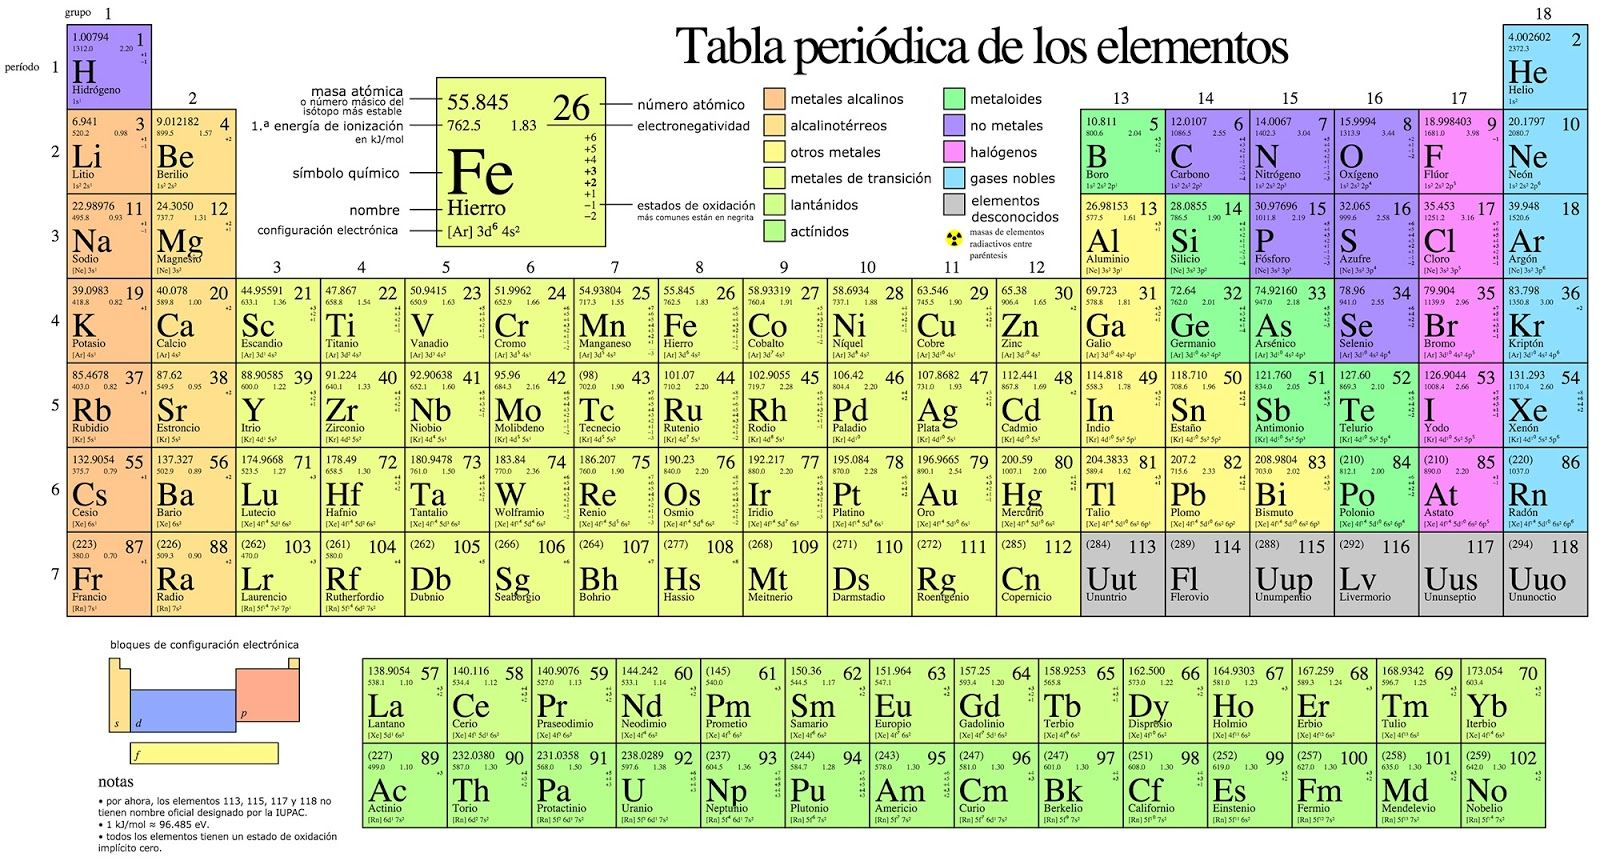
\includegraphics[width=\textheight,angle=90]{images/fig:tabla_periódica}
    \caption{Tabla periódica estándar}
    \label{fig:tabla_periódica_estándar}
\end{figure}

\newpage

\begin{figure}[H]
    \centering
    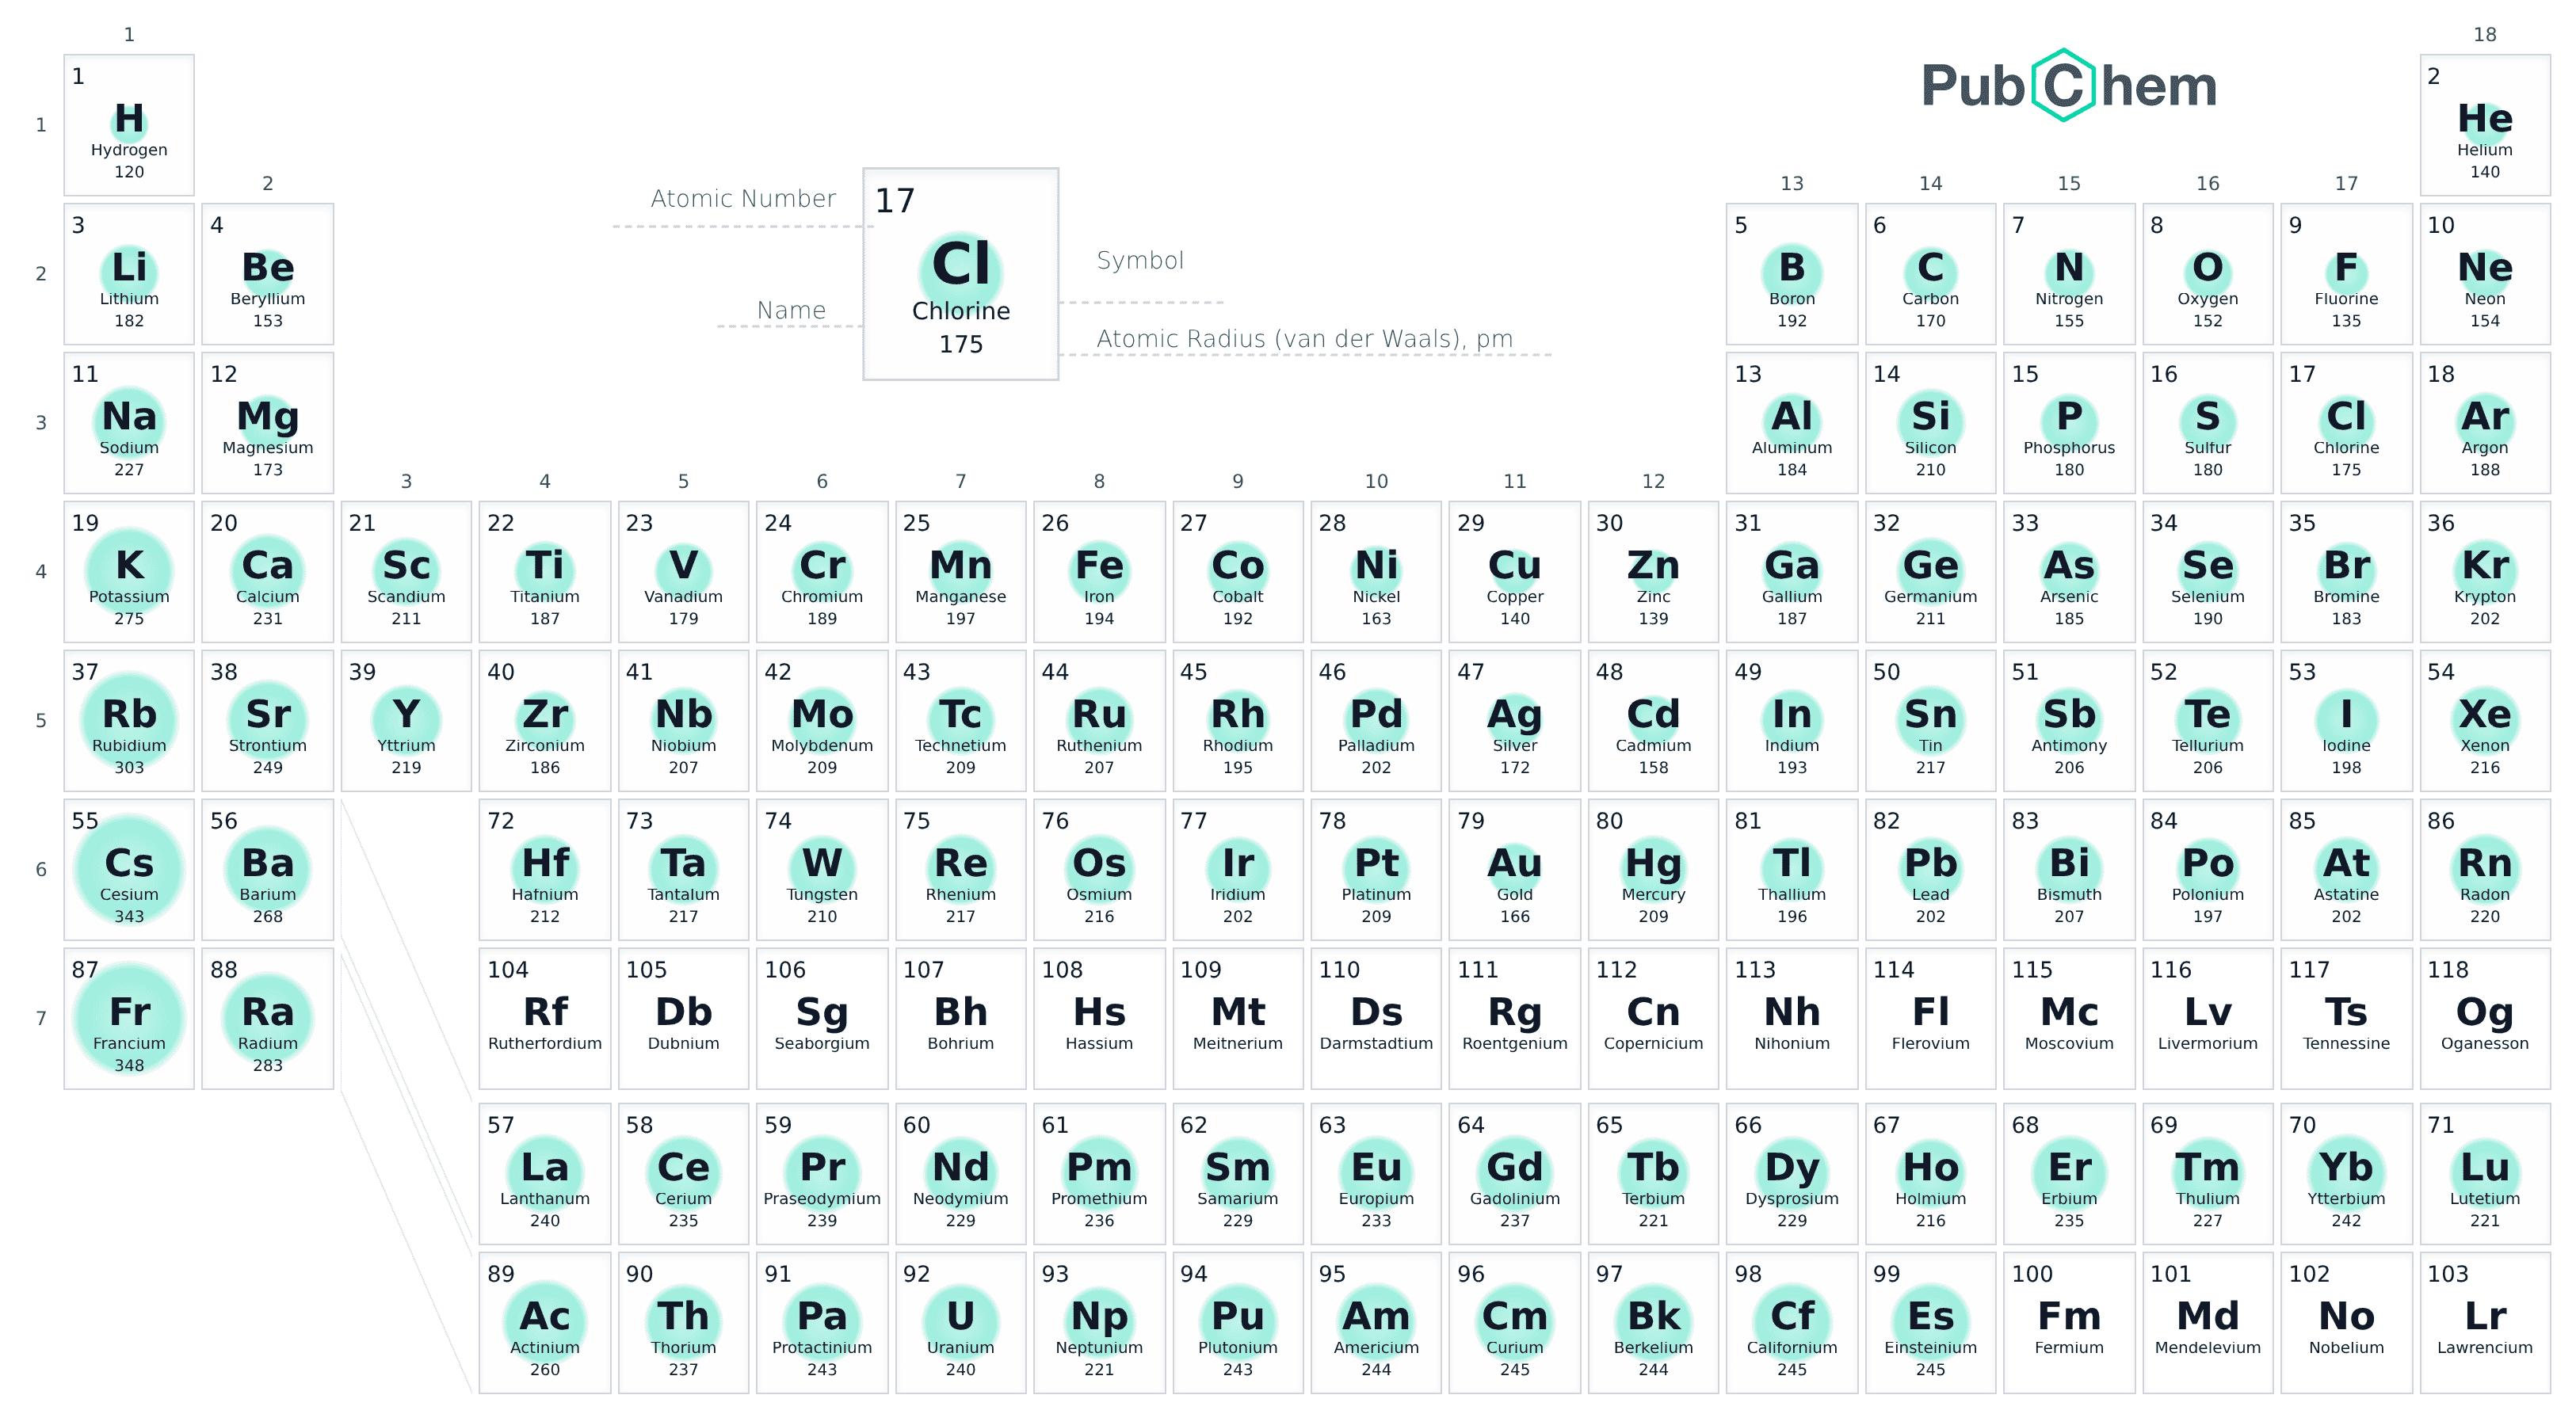
\includegraphics[width=\textheight,angle=90]{./images/fig:radio_atómico.png}
    \caption{Tabla periódica: Radio atómico por elemento.}
    \label{fig:tabla_radio_atómico}
\end{figure}

\newpage

\begin{figure}[H]
    \centering
    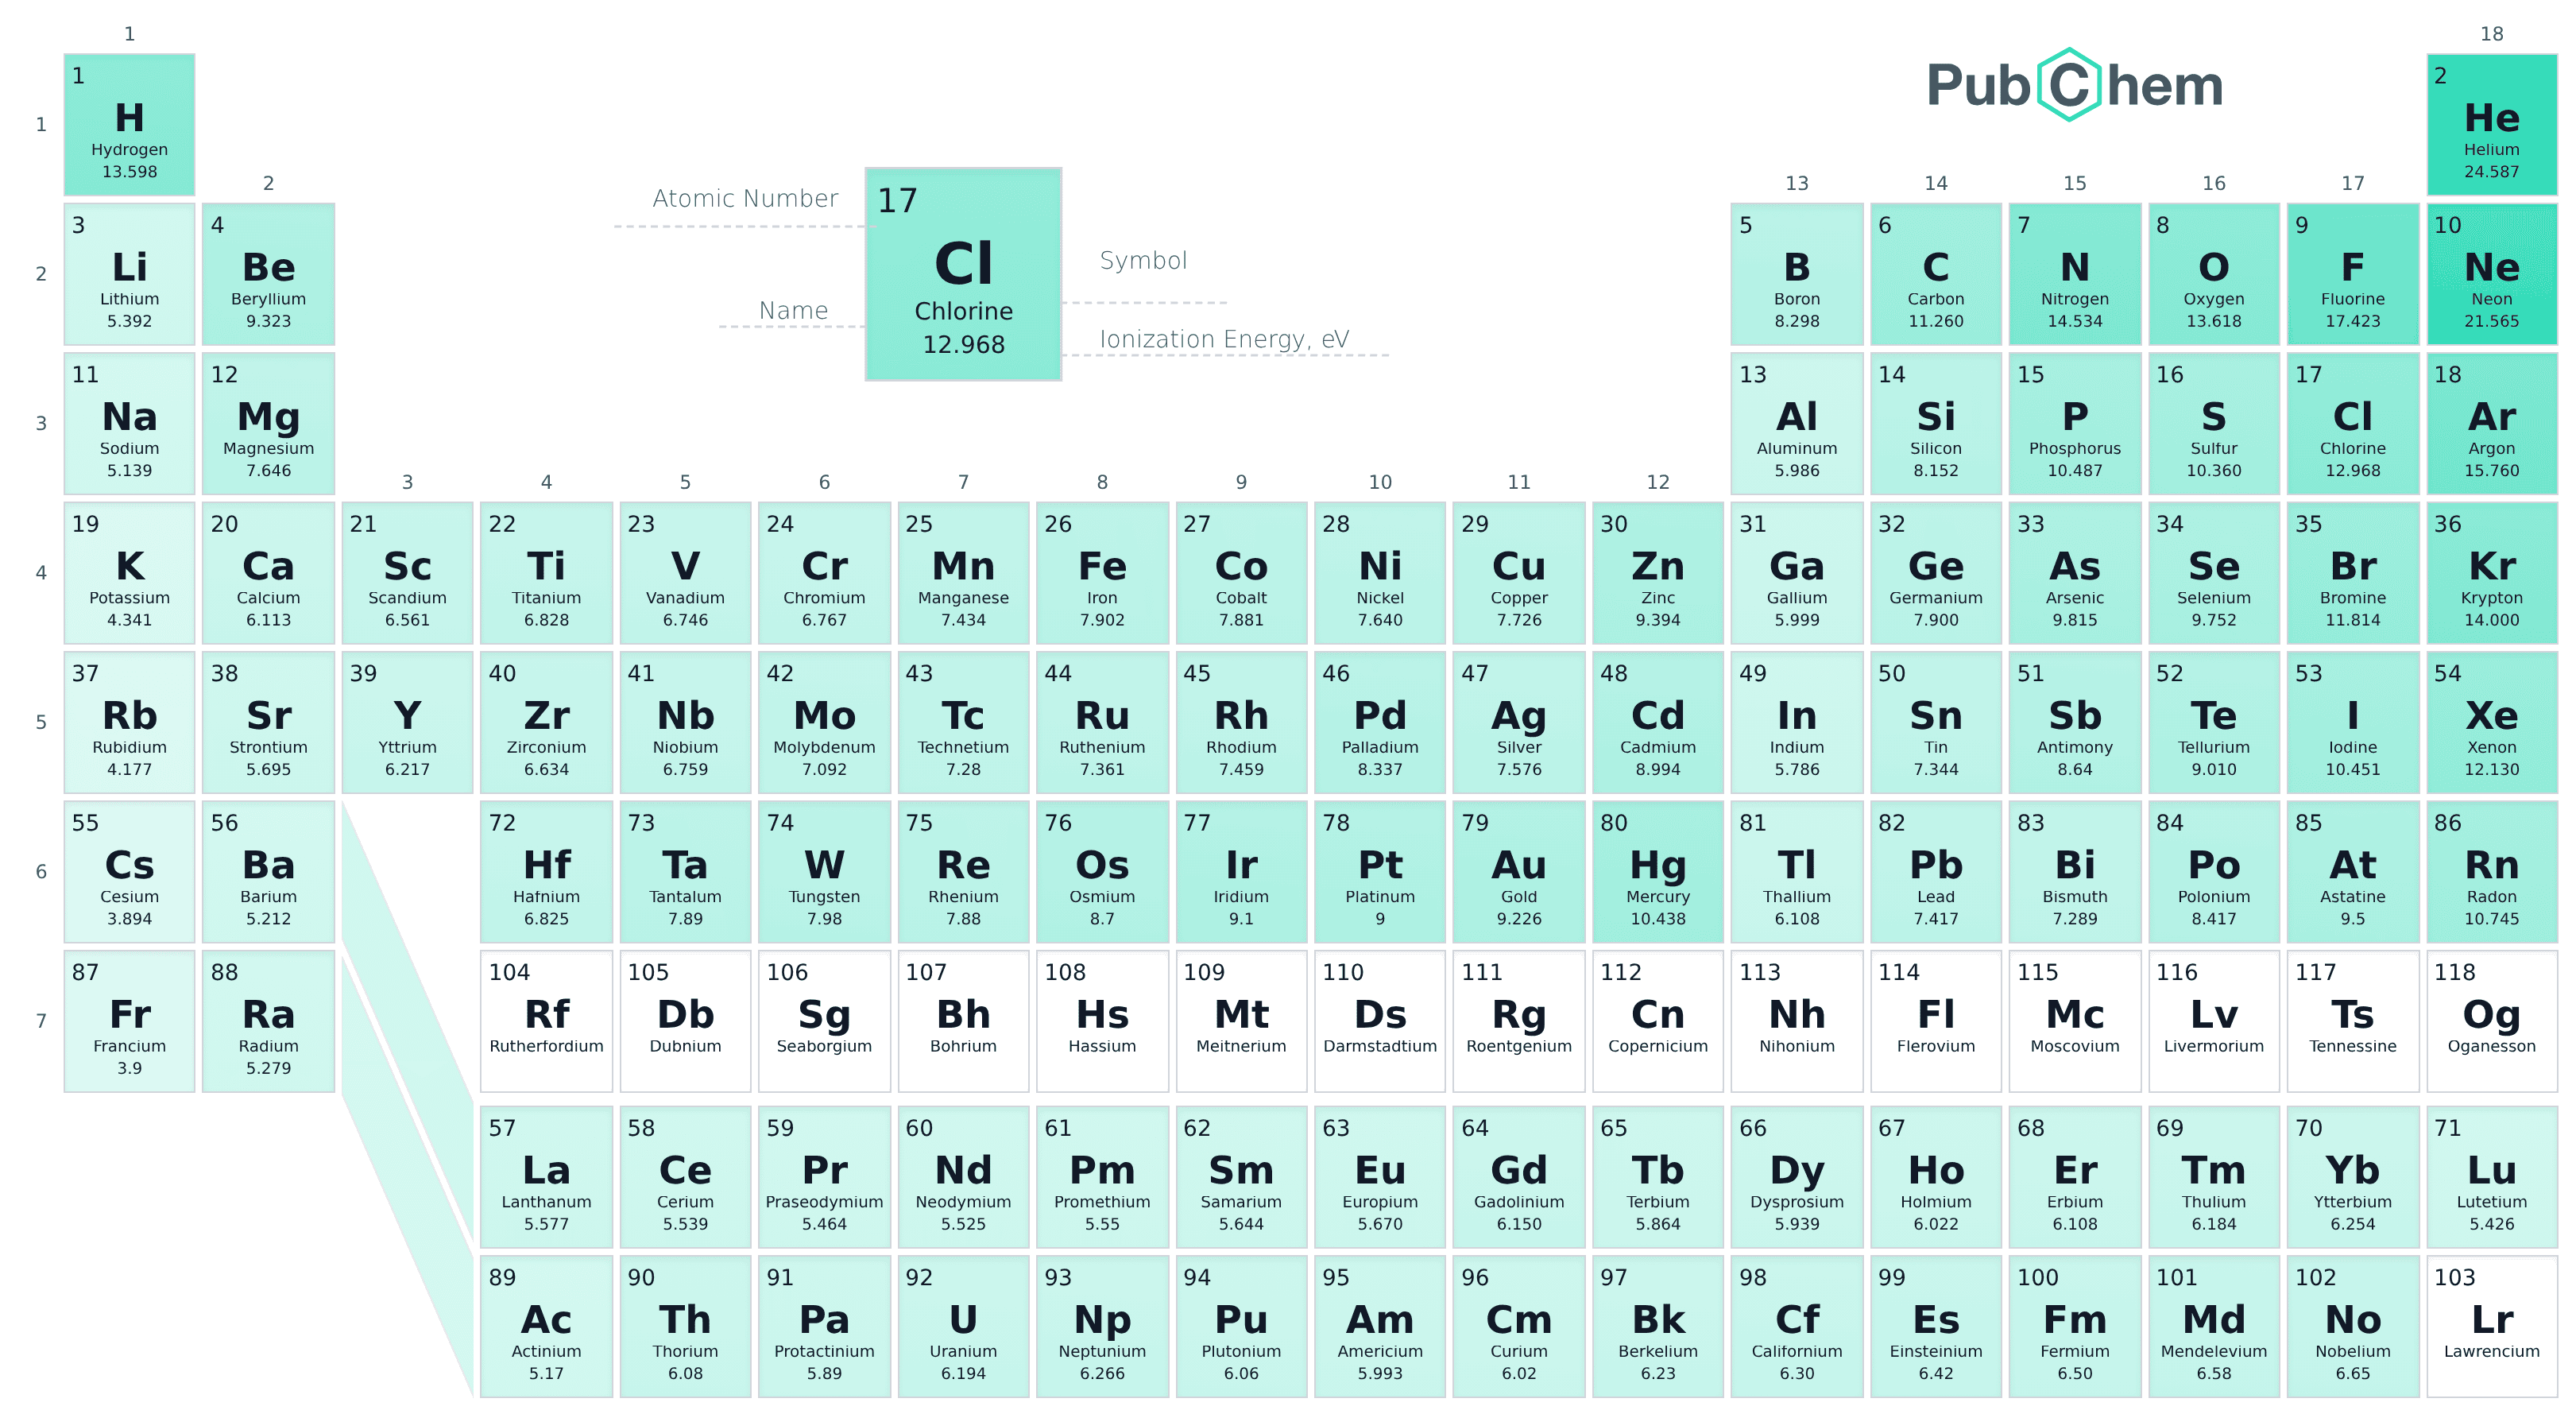
\includegraphics[width=\textheight,angle=90]{./images/fig:energía_de_ionización.png}
    \caption{Tabla periódica: Energía de ionización por elemento.}
    \label{fig:tabla_energía_de_ionización}
\end{figure}

\newpage

\begin{figure}[H]
    \centering
    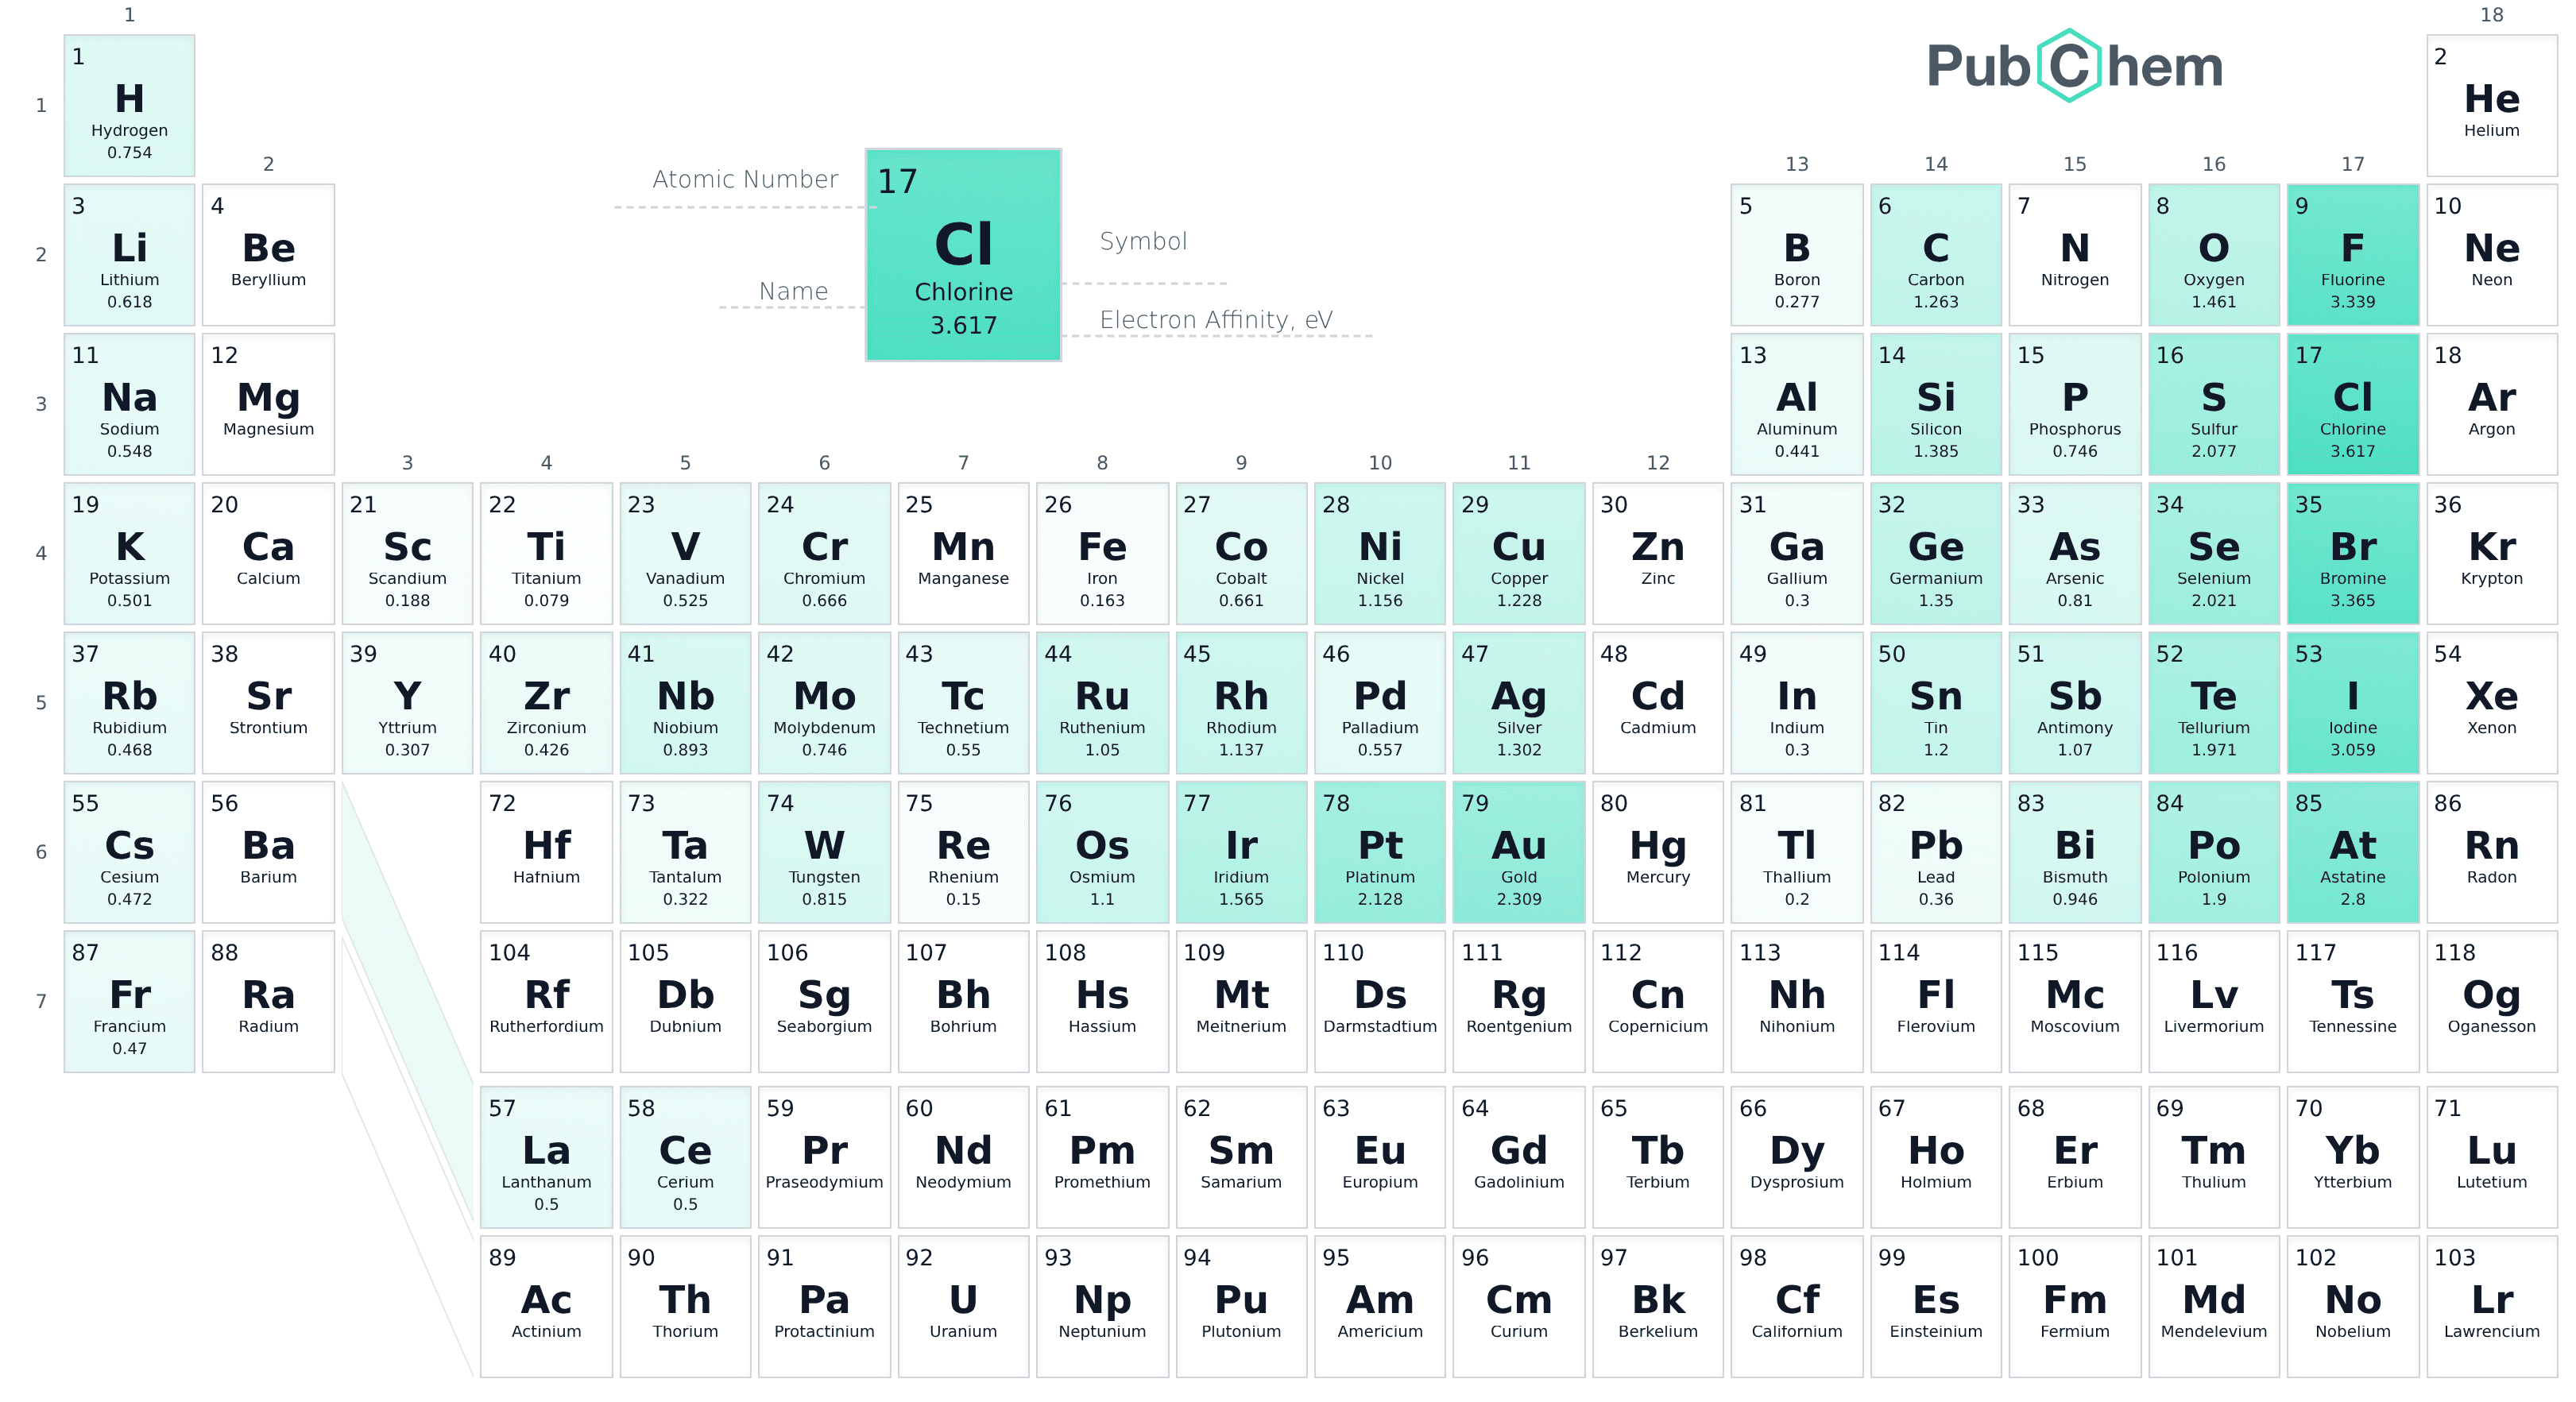
\includegraphics[width=\textheight,angle=90]{./images/fig:afinidad_electrónica.png}
    \caption{Tabla periódica: Afinidad electrónica por elemento.}
    \label{fig:tabla_afinidad_electrónica}
\end{figure}

\newpage

\begin{figure}[H]
    \centering
    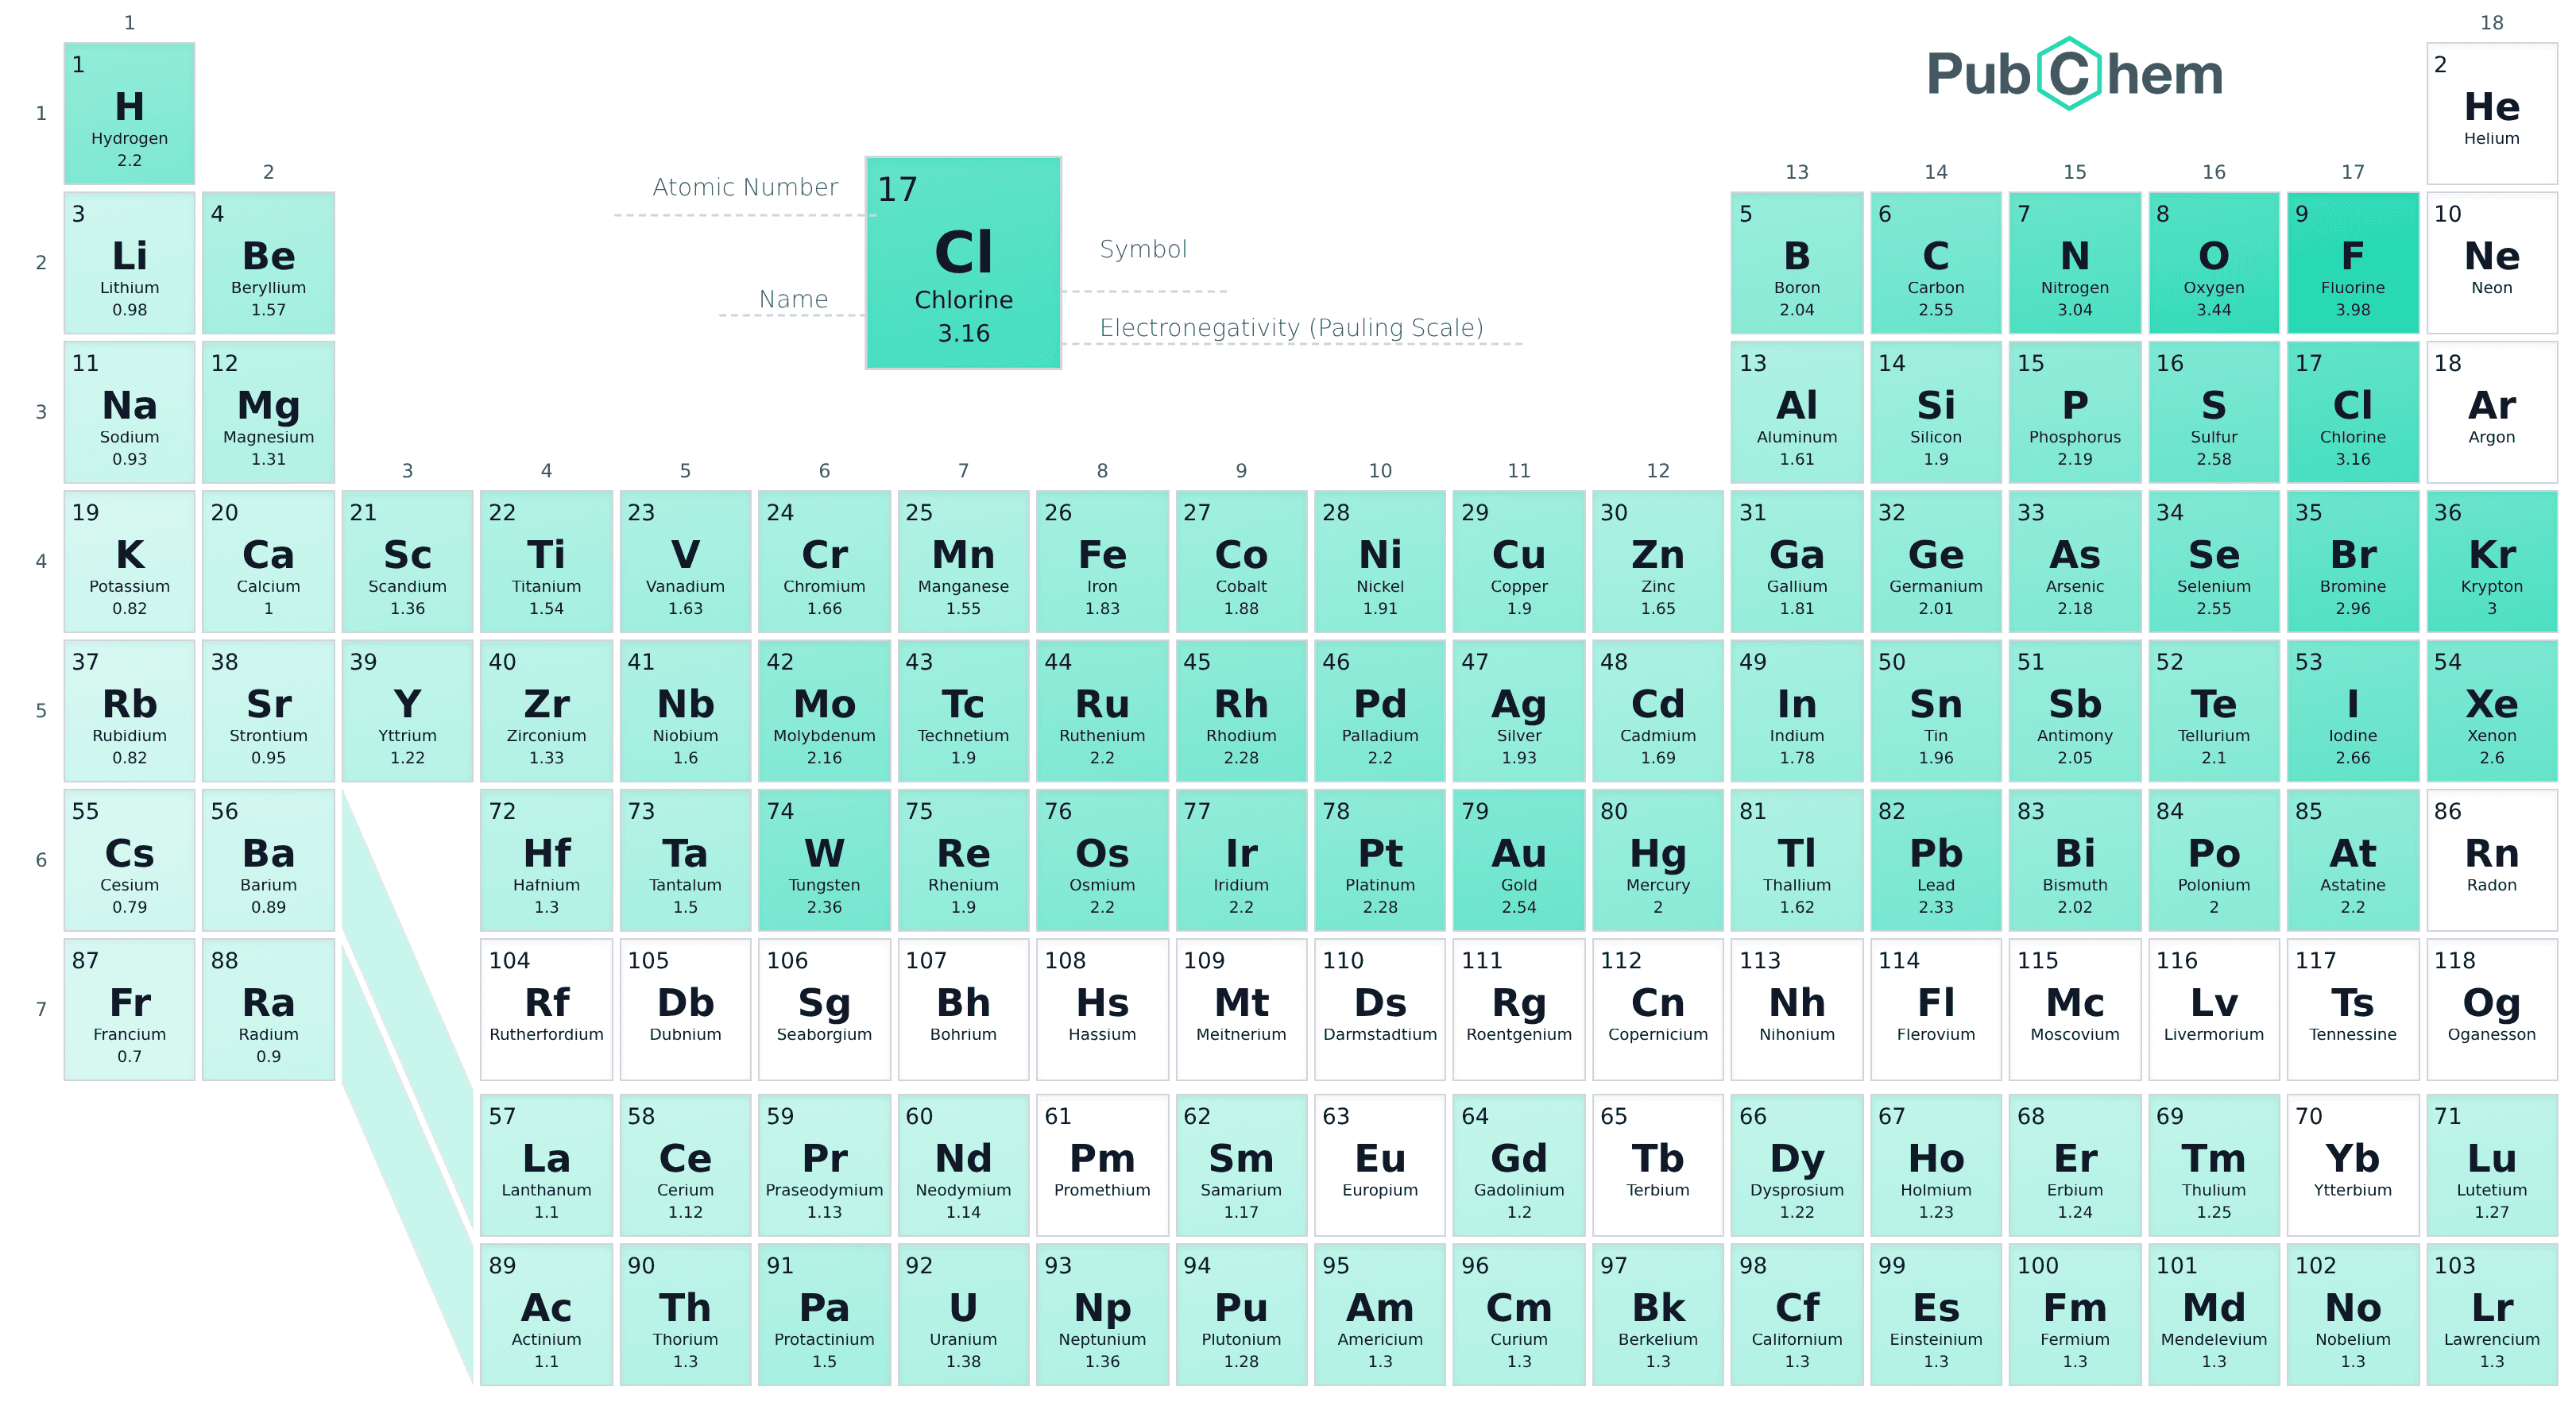
\includegraphics[width=\textheight,angle=90]{./images/fig:electronegatividad.png}
    \caption{Tabla periódica: Electronegatividad por elemento.}
    \label{fig:tabla_electronegatividad}
\end{figure}

\pagestyle{fancy}
\clearpage